\documentclass[12pt,a4paper]{article}
\usepackage[utf8]{inputenc}
\usepackage{graphicx}
\usepackage{float}
\usepackage{subcaption}
\usepackage[margin=1in]{geometry}
\usepackage{hyperref}
\hypersetup{
  pdfborder = {0 0 0}
}
\usepackage[
backend=biber,
style=alphabetic,
]{biblatex}

\addbibresource{PhSp.bib}

\graphicspath{{./PhSp/}}
\DeclareGraphicsExtensions{.pdf,.jpeg,.jpg,.png}

\usepackage{amsmath} % equations
\usepackage{fancyhdr} % nicer page header

\setlength{\parindent}{0pt} % no paragraph indents
\setlength{\parskip}{1em} % paragraphs separated by one line

\newcommand\experiment{N-Body Simulations with REBOUND} %%%%% experiment name
\newcommand\groupno{Group 3}       %%%%% group number
\newcommand\names{Pratyush Singh,\\
                  Proshmit Dasputpa\\}        %%%%% full names
\newcommand\expdate{07/03/2025}    %%%%% date of experiment day

\begin{document}
\begin{titlepage}
   \begin{center}
        \vspace*{3cm}
        \Huge{\experiment}
				
        \vspace{0.5cm}
        \LARGE{Lab course protocol}
				
        \vspace{3 cm}
        \Large{\groupno}
				
        \vspace{0.25cm}
        \large{\names}
				
        \vspace{2 cm}
        \Large{\expdate}
				
        \vspace{0.25 cm}
        \Large{Advanced lab course in astronomy\\
				Eberhard Karls Universit\"at T\"ubingen}
				
				\vspace{0.1 cm}
        \Large{WiSe 2024/25}
				
       \vfill
    \end{center}
\end{titlepage}

\pagestyle{fancy}
\fancyhf{}
\setlength{\headheight}{14.5pt}
\lhead{\groupno; \experiment}

\section*{Abstract}
This is optional, but never longer than half a page.

\tableofcontents
\newpage

\setcounter{page}{1}
\pagestyle{fancy}
\fancyhf{}
\rhead{\thepage}
\lhead{\groupno; \experiment}

\section{Introduction}\label{sec:intro} % labels allow references, particularly important for figures and tables
In the experiment, we will use the 80 cm telescope of the IAAT to study photometry and spectroscopy. These two topics are fundamental to observational astronomy 
and are used to study the properties of stars, galaxies and other bodies. In photometry, we aim to determine the brightness of several stars in the star cluster M37 in 
the B and V filters which will be used to determine the age and distance to the cluster. In spectroscopy, we will look at the spectrum of one (or both) of the stars of 
the Castor binary system and identify the $H\alpha$ spectral line (and more).


\section{Theory}\label{sec:theory}
\subsection{Telescope}
  Telescopes are used in observing the EM radiation emitted by distant sources. Telescopes collect light from a certain direction and are used to apply an angular magnification to the image. The two major types of telescopes are 
  the lens telescope (the refractor) or the mirror telescope (the reflector). The amount of light that a telescope can gather depends on the `aperture' of the telescope $D$. The ratio of this and the focal length
  $F$ is the aperture ratio $F/D$. A telescope with a higher aperture ratio will produce a brighter image. The magnification of the telescope is determined by the ratio of the main mirror focal length $F$ and the eye piece focal length
  $f$. i.e. $M = F/f$. 
  \\
  The resolving power of a telescope is its ability to distinguish between two nearby sources and is defined by the Rayleigh criterion:
  \begin{equation}
    \alpha = 1.22 \frac{\lambda}{D}
  \end{equation}

  Unfortunately due to atmospheric effects, the resolving power is slightly worse and is limited to $\alpha = \lambda/D$. For a telescope with an aperture of 80 cm, the resolving power
  at $\lambda = 5700 \AA$  is \dots.
  \subsubsection{The 80 cm Telescope}
    The 80 cm telescope is located in Sand, Tübingen and was built in 2003. It is a mirror telescope in Cassegrain configuration with Nasmyth focus. It has an aperture of 80 cm and 
    a focal length of 6.4 m. For slewing, the telescope is mounted on an equatorial open fork mount and can move to focus on any point in the sky in its line of sight.
    \begin{figure}[H]
      \centering
      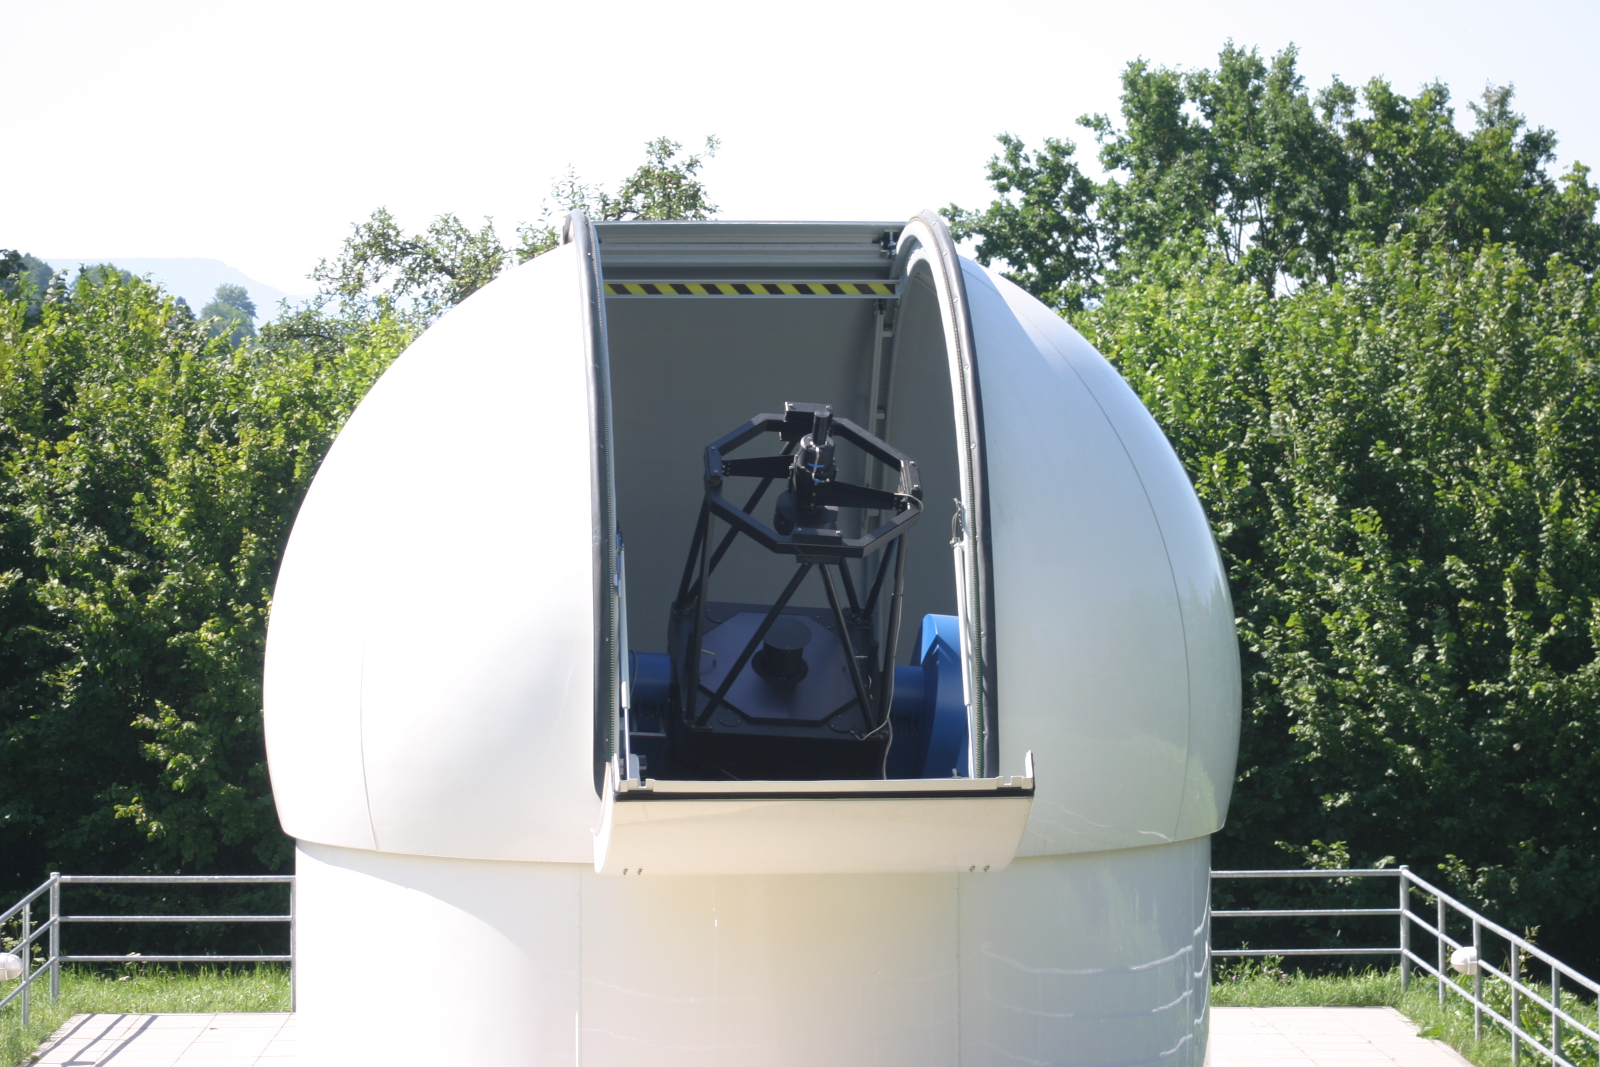
\includegraphics[width=0.5\textwidth]{./Pictures/2004_img_0962.jpg}
      \caption{The 80 cm telescope at the IAAT.}
      \label{fig:80cm}
    \end{figure}
    In figure \ref{fig:80cm_lp} we can see the path light has to travel to reach the focus points. The starlight enters from above and is reflected by the primary mirror towards the 
    secondary mirror. It reflects back the light towards a plain mirror which focuses the light on either the left or the right focus. This configuration (Cassegrain-Nasmyth) allows a smaller size of the telescope
    (around 3 m) for a larger focal length of 6.4 m. The Nasmyth focus also is beneficial for mounting heavy instruments that don't need to be moved with the declination axis. 
    \begin{figure}[H]
      \centering
      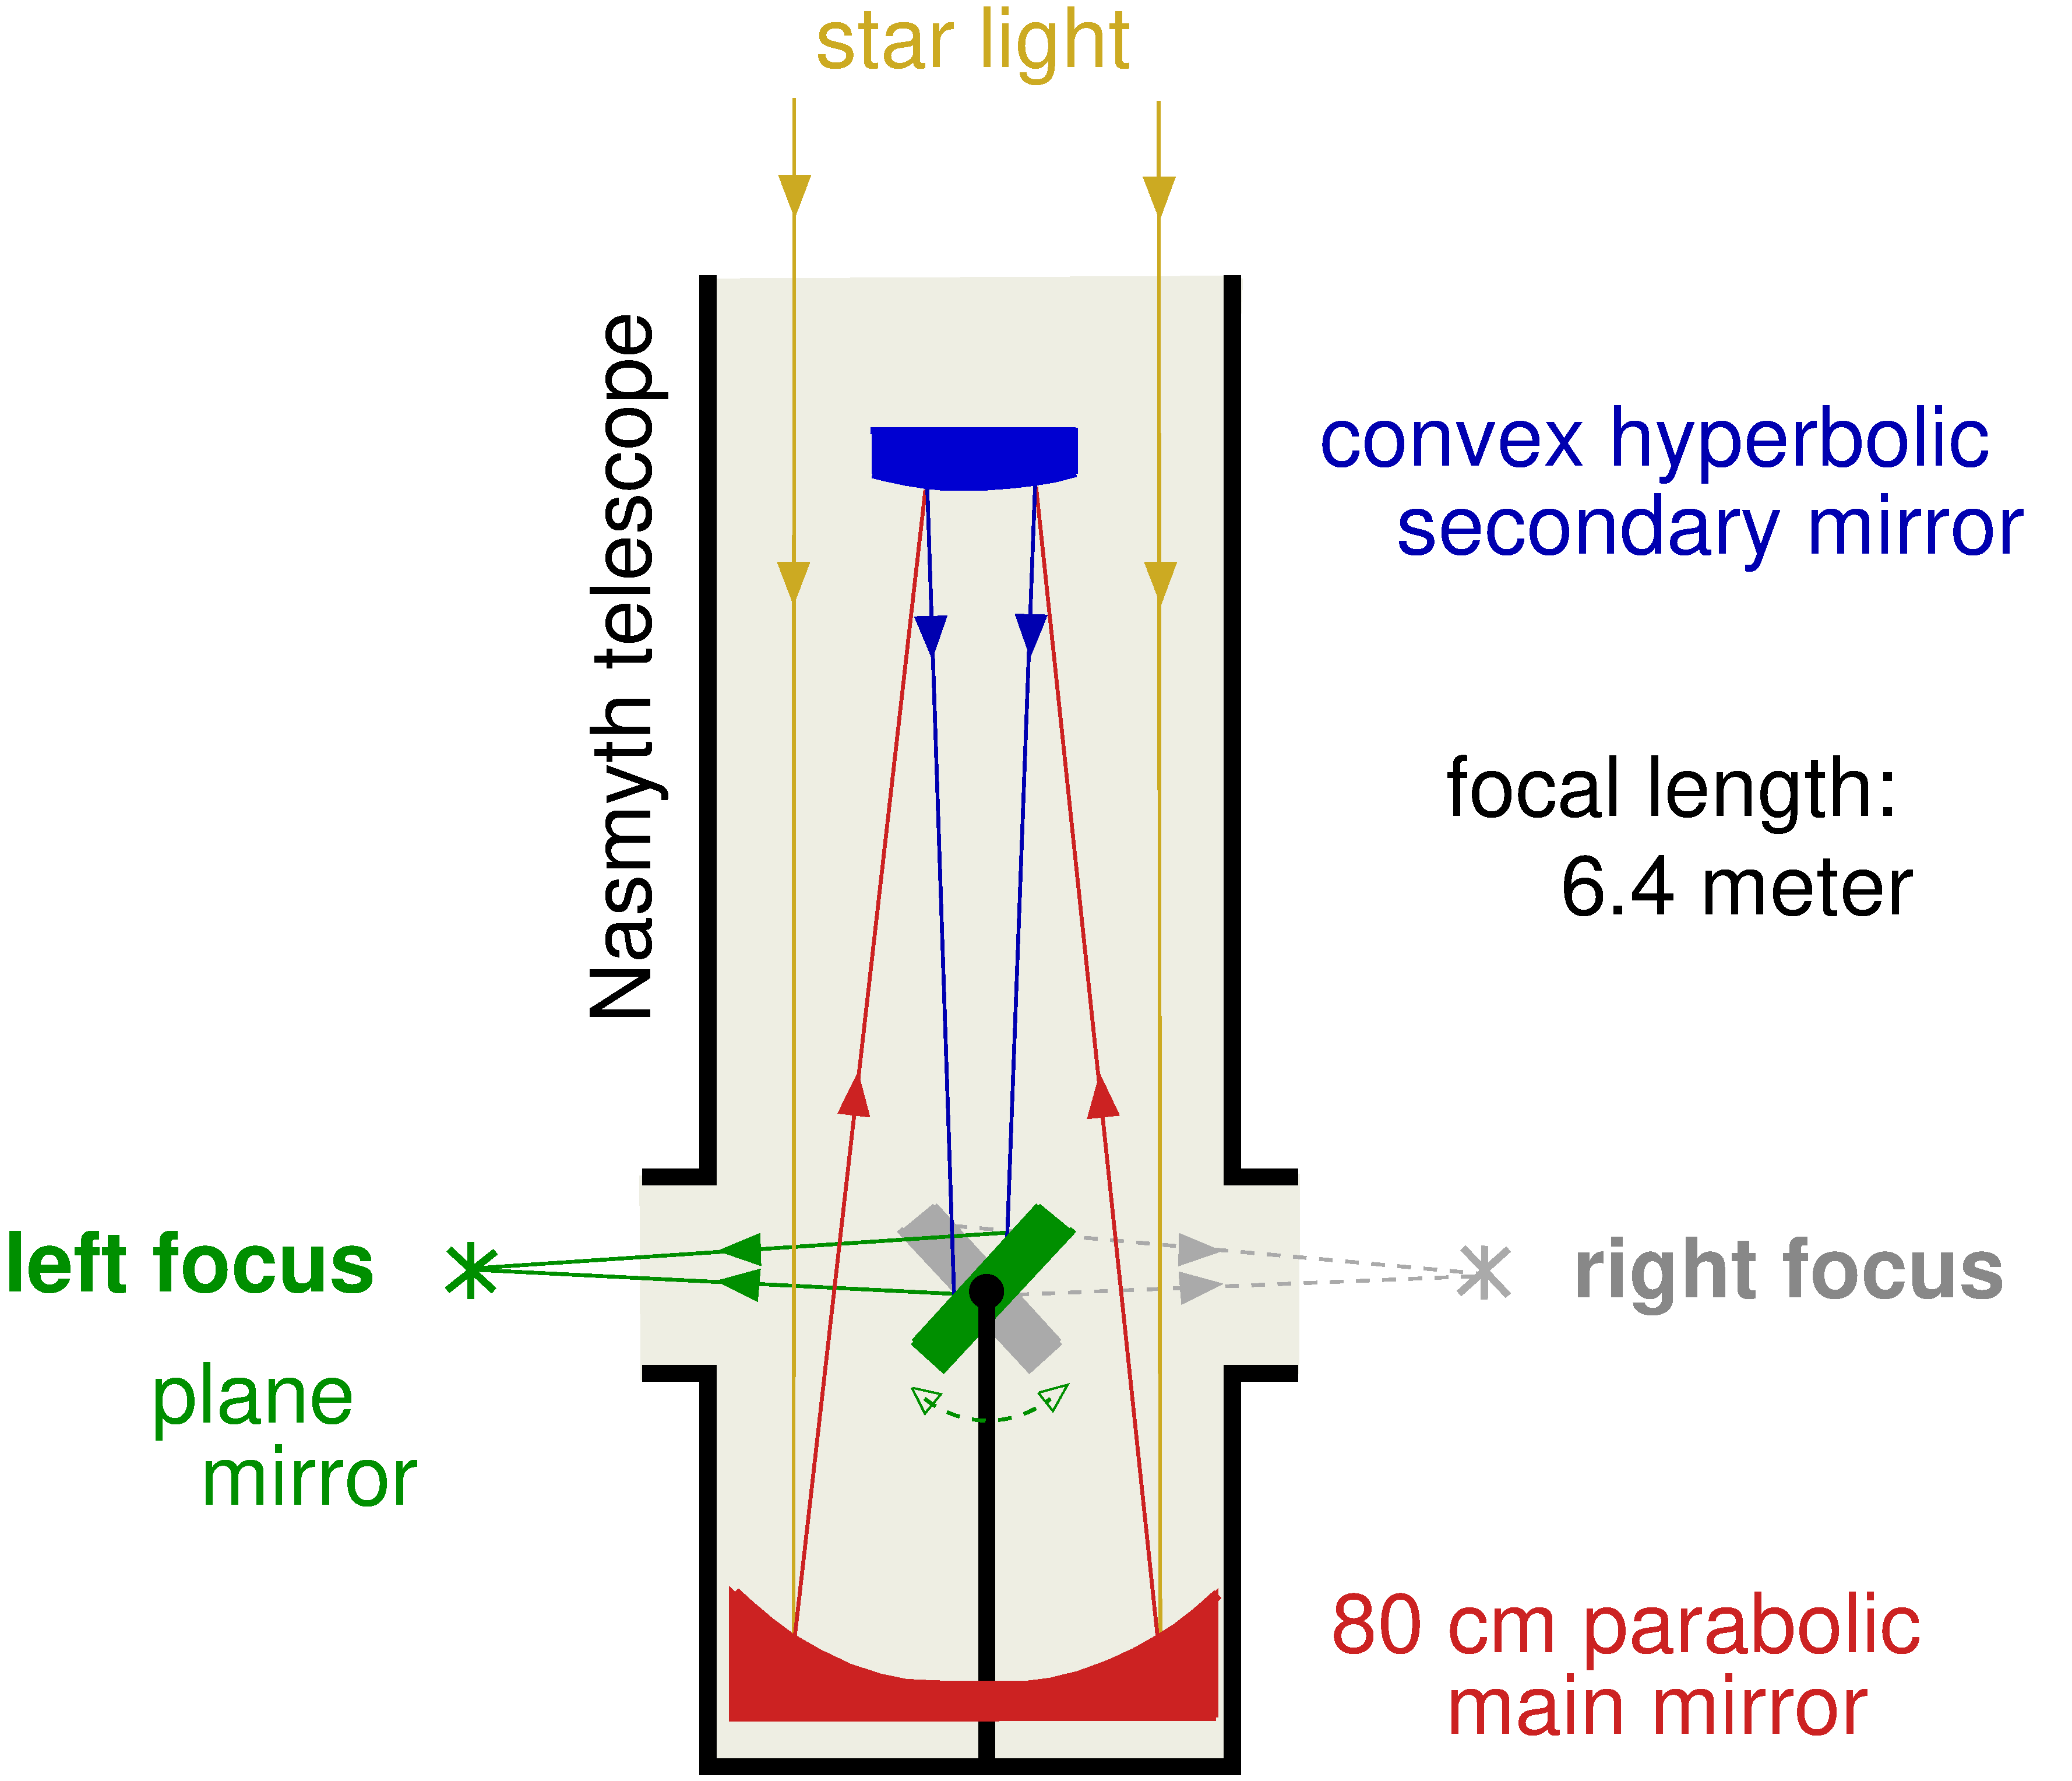
\includegraphics[width=0.5\textwidth]{Pictures/Nasmyth2.pdf}
      \caption{The light path of the 80 cm telescope.}
      \label{fig:80cm_lp}
    \end{figure}

  \subsection{CCD}
  \subsection{Photometry}
  \subsection{Spectroscopy}
    Studying the spectrum of stars can reveal information like their temperature, composition and their physical properties. The absorption and emission lines present 
    in a spectra caused by certain transitions in the elements present in the star and help in identifying its chemical composition. These lines are used to group
    stars into different spectral classes. \\

    \subsubsection{Star Classification}
    Using the Morgan and Keenan system, stars are classified depending on their spectrum and their luminosity. Both these parameters are required for classification since 
    stars st different stages of their life can have the same spectral class, while their sizes may strongly differ. Therefore to make their classification unambiguous `luminosity class' 
    is also used. The luminosity classes are defined in the figure \ref{fig:MK}.
    \begin{figure}[H]
      \centering
      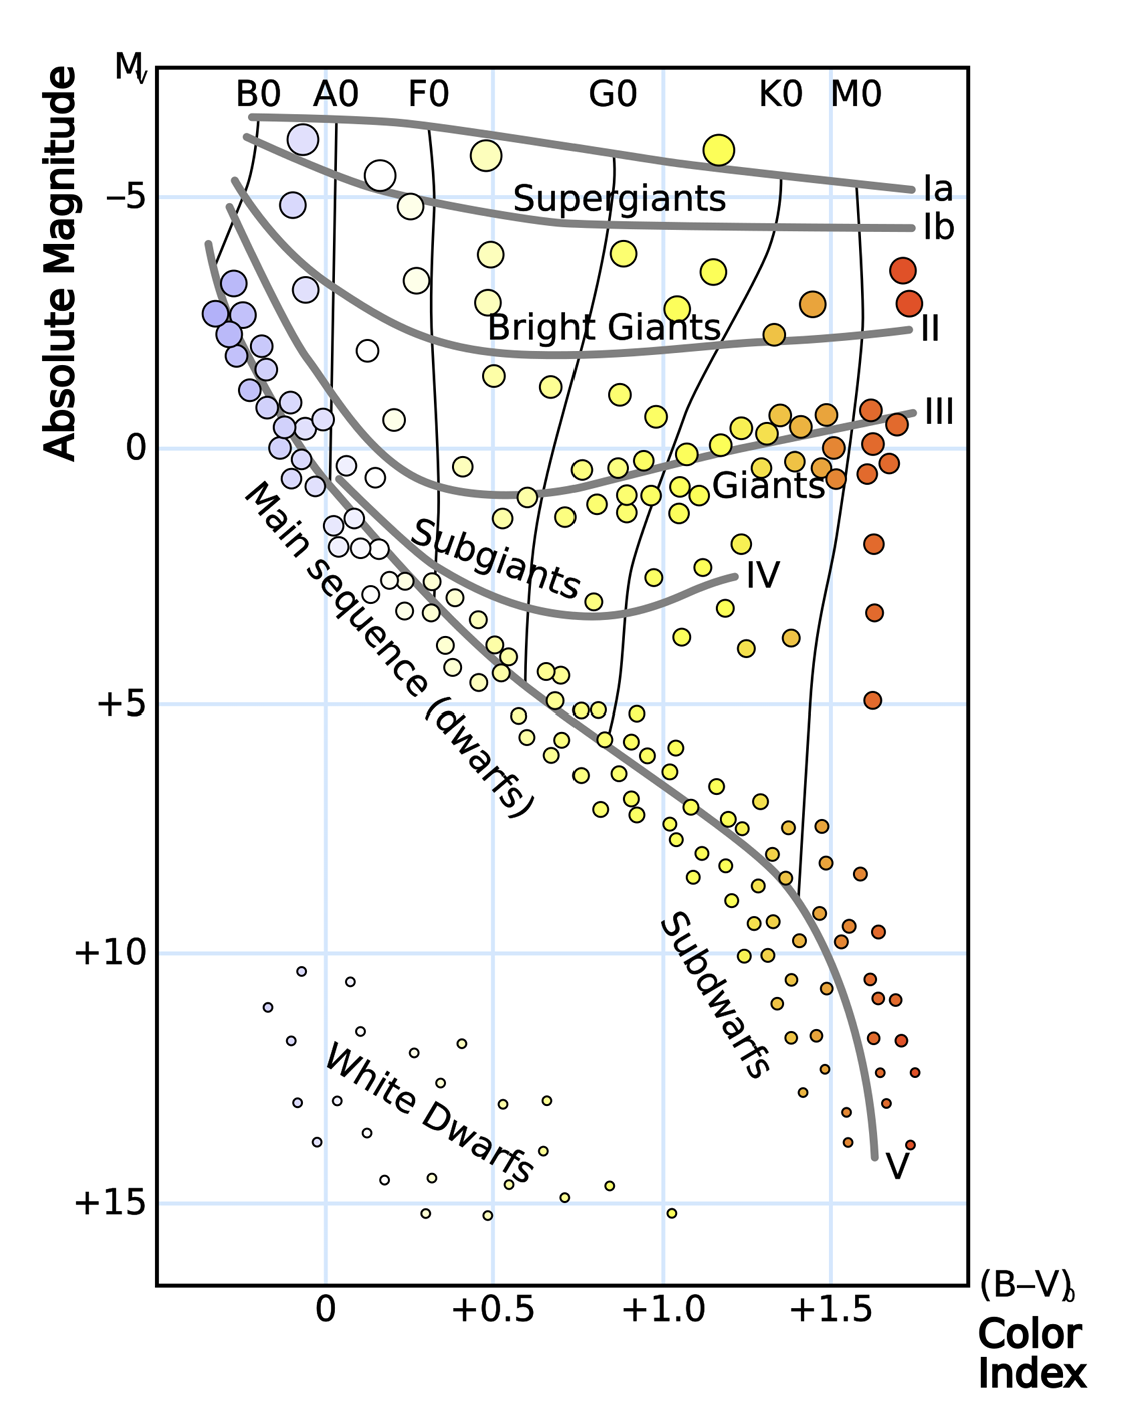
\includegraphics[width=0.5\textwidth]{Pictures/HRD_lum_class.png}
      \caption{HRD diagram with Luminosity Classification}
      \label{fig:MK}
    \end{figure}

    Stars are classified into a `spectral class' based on the strength of their various spectral lines. The spectral class of a star is also a direct measure of the temperature of the star. The spectral classes are labelled
    `O', `B', `A', `F', `G', `K', `M', `L' and `T' in decreasing order of temperature. Each is further split into 10 sub classes from 0 to 9. \\
    \begin{table}[H]
      \begin{tabular}{||c|c|c||}
        \hline
        Spectral Type & Temperature Range (K) & Distinguishing Features\\
        \hline
        \hline
        O	&> 25,000K	&H; HeI; HeII\\
        B	&10,000-25,000K	&H; HeI; HeII absent\\
        A	&7,500-10,000K	&H; CaII; HeI and HeII absent\\
        F	&6,000-7,500K	  &H; metals (CaII, Fe, etc)\\
        G	&5,000-6,000K  	&H; metals; some molecular species\\
        K	&3,500-5,000K	  &metals; some molecular species\\
        M	&$\leq $3,500K	metals;& molecular species (TiO!)\\
        C	&$\leq $ 3,500K	metals; &molecular species (C2!)\\
        \hline
      \end{tabular}
      \caption{Temperature and Absorption lines at different spectral Classes\cite{Spectral_Classification}}
    \end{table} 
    Stellar plasma below the photosphere creates a black body spectrum. The temperature at which this peaks is the effective temperature of the star. As the temperature in the outer regions of the photosphere is lower,
    different elements absorb parts of the light coming from deeper in the star and create the absorption lines. These lines are highly dependent on the effective temperature and the elements present in the photosphere.
    \\
    The most abundant absorption lines are usually the $H_\alpha$, $H_\beta$, $H_\gamma$ and $H_\delta$ lines of the Balmer series. These are caused by ionized hydrogen, which is the most abundant elements in stars.
    Hydrogen lines are most abundant in A type stars. For G type and cooler stars, Calcium lines are more dominant. Figure \ref{fig:abs_lines} shows this in more detail.
    \begin{figure}[H]
      \centering
      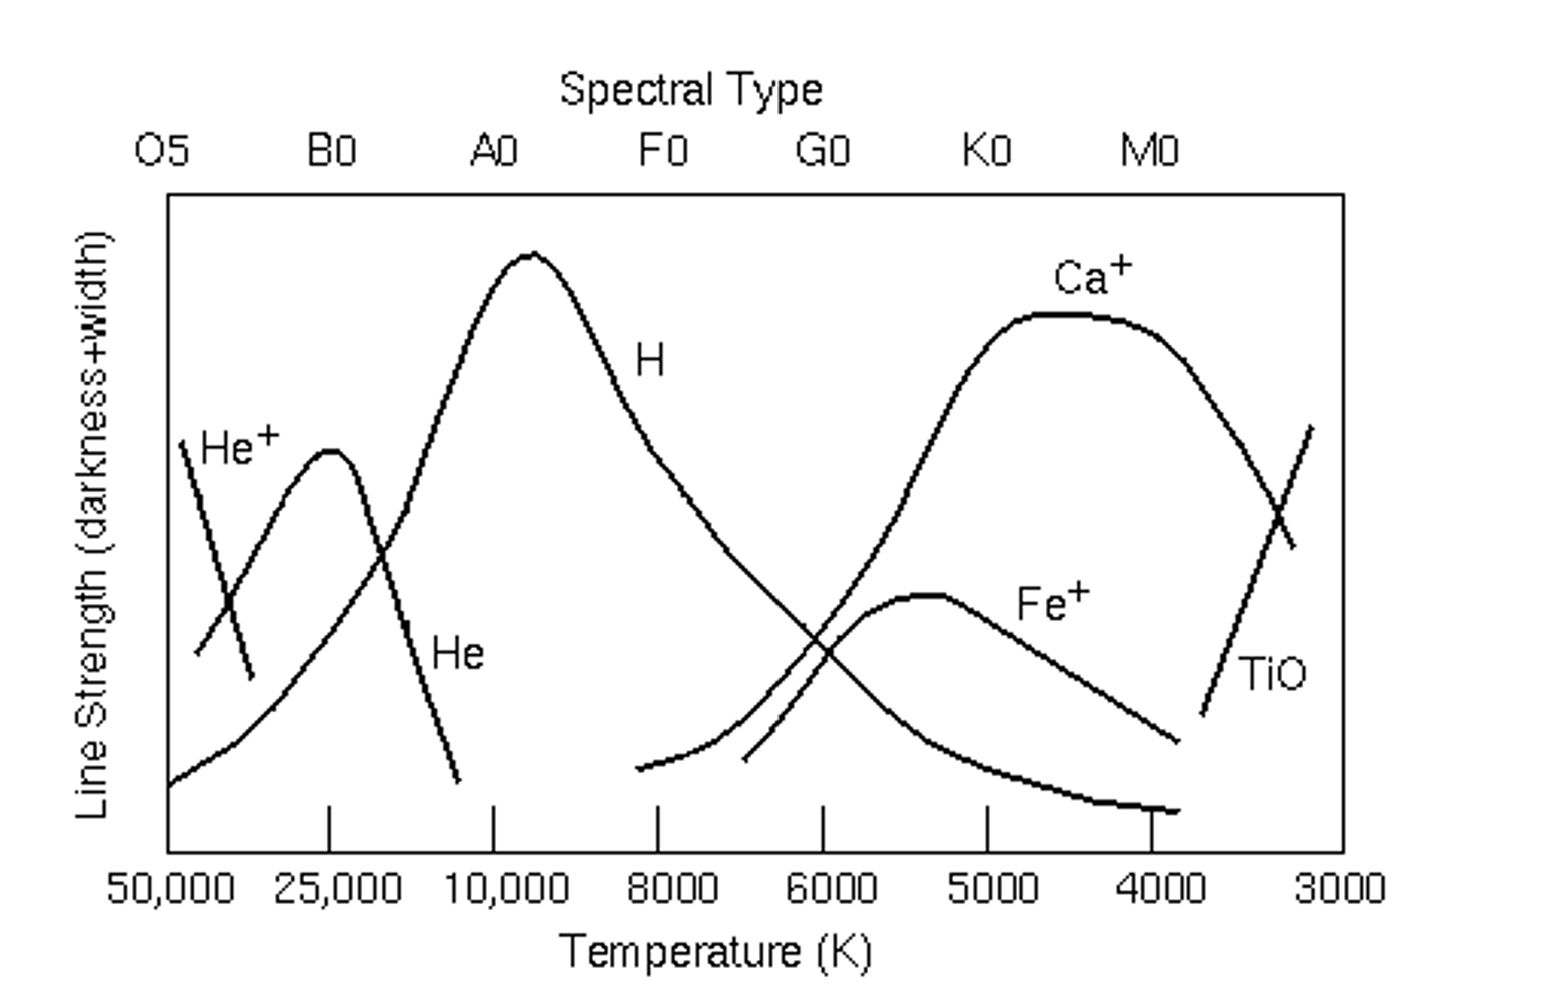
\includegraphics[width=0.75\textwidth]{Pictures/Line_strength.png}
      \caption{Strength of absorption lines at different temperatures}
      \label{fig:abs_lines}
    \end{figure}
    Figure \ref{fig:spec_class} shows the spectra of stars of different sizes. Most of the spectral features are found in UV, hence spectroscopy is very popular in UV astronomy. 
    
    \begin{figure}[H]
      \centering
      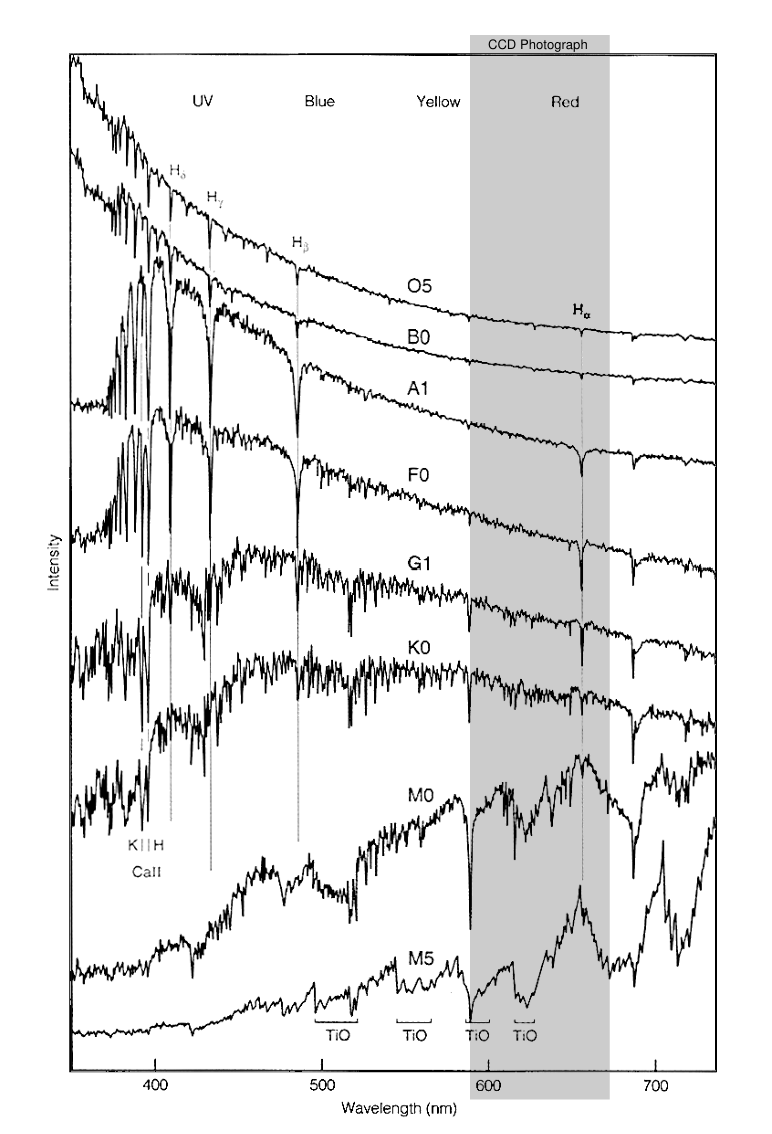
\includegraphics[width=0.75\textwidth]{Pictures/Spectral_class.png}
      \caption{Spectra of stars of different spectral classes.}
      \label{fig:spec_class}
    \end{figure}
\section{Experiment} 
\subsection{Spectroscopy}
    We observed the spectrum of one (or both) stars in the Castor binary system. To observe the spectra, the 10C spectrograph was mounted on the 
    left focus of the 80 cm telescope. The spectrograph uses a CCD camera to obtain the spectral image of the star. To control the spectrograph, `Maxim DL'
    software is used. 
    \subsubsection{Recording the Data}
      In order to obtain the spectra, the steps are listed below:
      \begin{enumerate}
        \item The telescope is powered on and the operation software is started on the `Telescope Computer', `Navigation and Observation Computer' and the `Spectral Analysis Computer'.
        \item The calibration lamps and the CCD of the spectrograph are powered on.
        \item Adjust the focus of the CCD. This must be set up manually directly at the spectrograph by following the markings on the camera. When mounting the spectrograph, be careful not To
              touch the focus dial.
        \item The telescope is slewed to the target star. Out of focus, the star will appear as a donut shaped object. The focus is manually adjusted until we observe a star like object(s).
        \item When the calibration lamps are on, the slit is visible between the two red discs that appear in the eyepiece. The telescope is slewed slightly until one of the stars is directly on the slit. 
        \item The spectral image can now be taken by the spectrograph. 
      \end{enumerate}

      \begin{figure}[H]
        \centering
        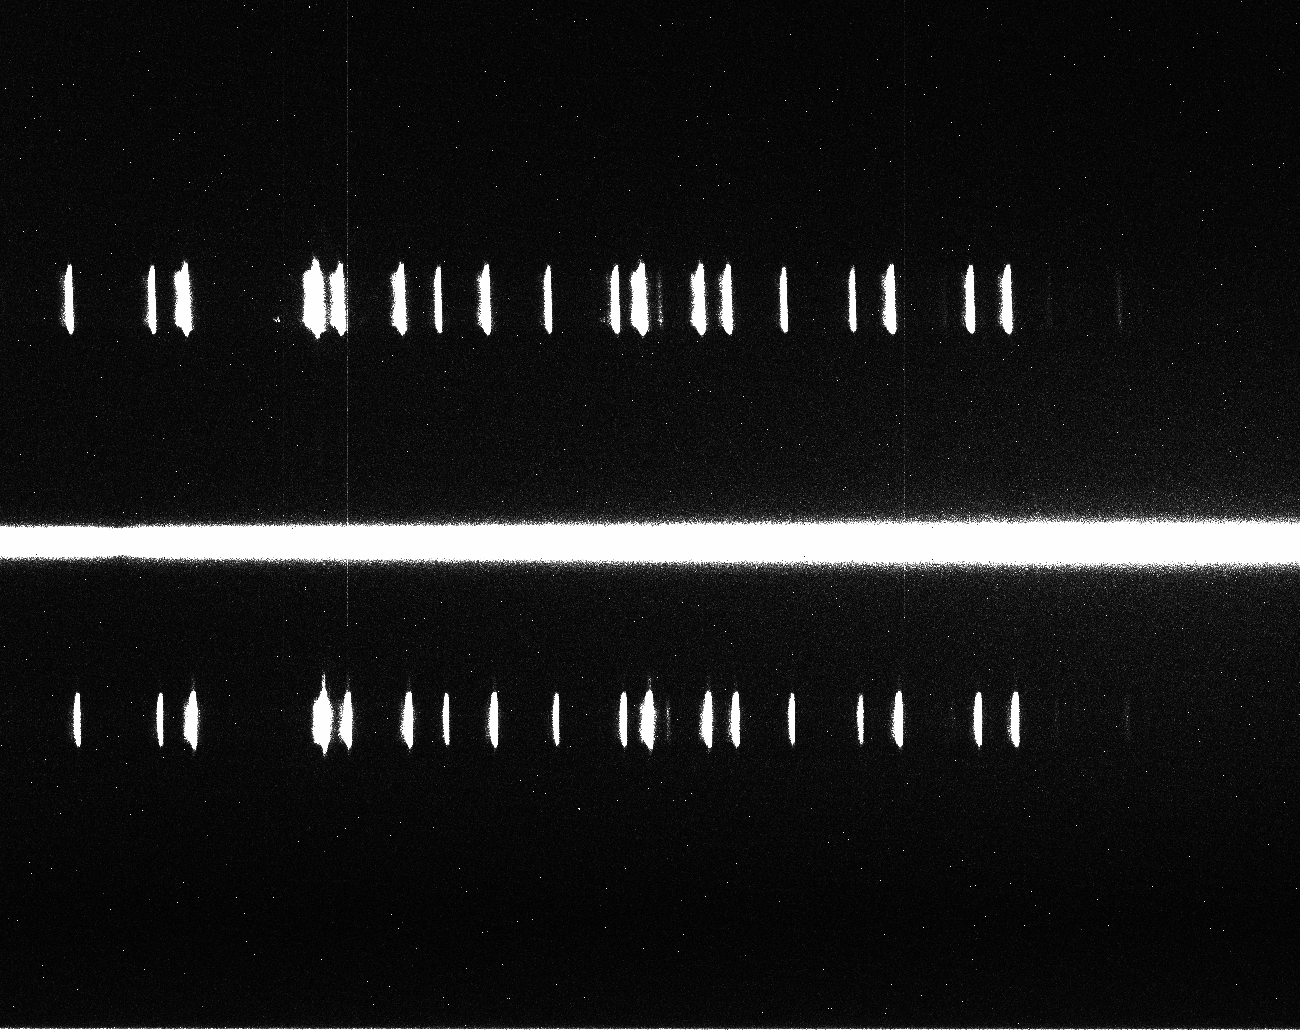
\includegraphics[width=0.75\textwidth]{Pictures/spectrum_image.png}
        \caption{Spectral image of the Castor binary system obtained using the SX-HX9 CCD camera of the 10C spectrograph and the 80 cm telescope. 
        We observe the top and bottom calibration lines and the star spectrum in the middle. Not much is directly visible in the image except possibly the $H_\alpha$ line}
        \label{spectrum_img} 
      \end{figure}
    \subsubsection{Data Analysis}
      The obtained spectral image is analysed using the `Spec-Analyser' software. 
\section{Conclusions}
An important section in which you should critically review the experiment and its results. Mention also parts that did not work out as expected, but keep a neutral to positive view. This can span from a few sentences to half a page.

\setcounter{secnumdepth}{0}

\printbibliography
\appendix
\section{Appendix}

Please attach here your original handwritten notes and other documents created during the experiment.

\end{document}

